
%%%%%%%%%%%%%%%%%%%%%%%%%%%  3  %%%%%%%%%%%%%%%%%%%%%%%%%%% 
\section{High performance on-chip differential signaling using passive compensation for global communication \cite{zhang2009high}} \label{ss:zhang2009high}
%%%%%%%%%%%%%%%%%%%%%%%%%%%  3  %%%%%%%%%%%%%%%%%%%%%%%%%%% 

\begin{figure}	\centering
	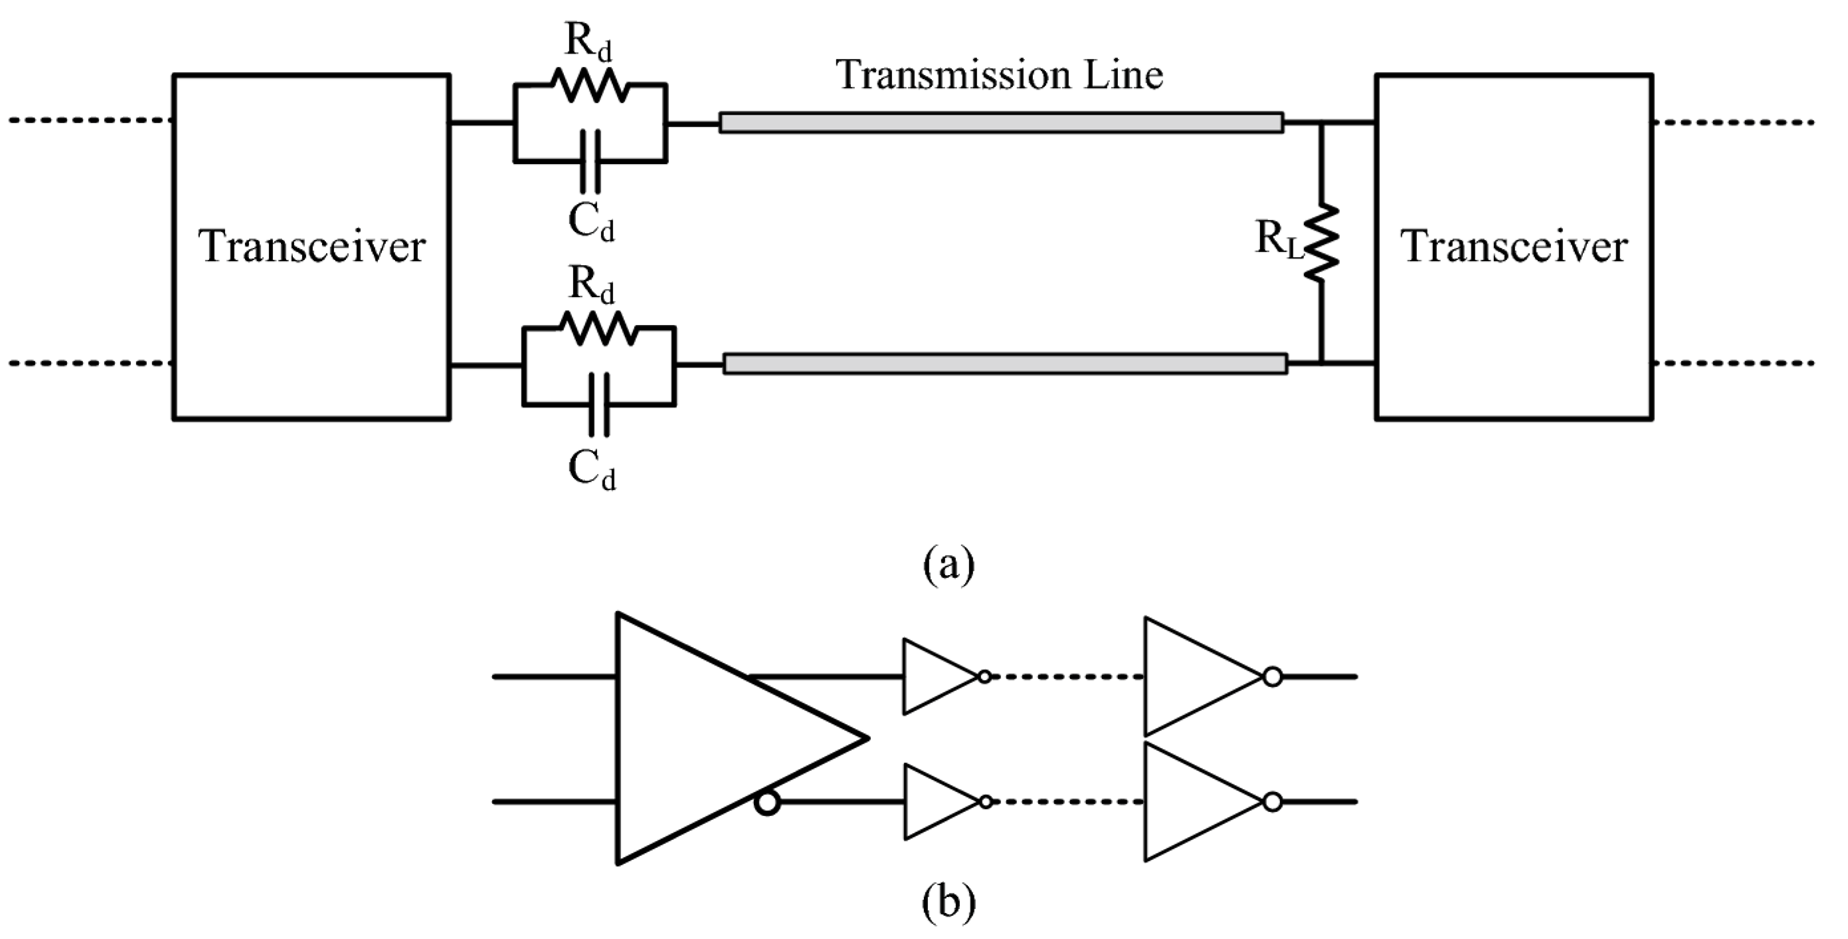
\includegraphics[width=0.95\linewidth]{Figures/Rep3Overview.png}
	\caption{Proposed signaling schema for global wiring: (a) one stage structure; (b) Sense Amplifier + inverter chain structure, Source: \cite{zhang2009high}.} 
    \label{fig:rep3:overview}
\end{figure}

The interconnect of a chip is regarded one of the most critical factors in the determination of performance and power consumption according the ITRS (International Technology Roadmap for Semiconductor) roadmap.
% MISSCHIEN ZIN VERANDEREN DIRECT OVERGENOMEN
For instance, the \textit{1 mm} global RC wire delay (at 45 \textit{nm} technology) is 385 \textit{ps} while the 10 level FO4 delay is below 200 \textit{ps}.
Traditionally the interconnect delay problem is dealed with by implementing a buffer (\textit{buffer insertion} also known as \textit{repeated RC wires}).
However, this introduces a power overhead, i.e. approximately half of the dynamic power is dissipated by the repeaters.

\motive
The use of \accs{otl} deliver signals with speed of light and consumes less power than repeaters, but the \acc{isi} can be a problem for performance.

\objective
A high performance on-chip global signaling with passive compensation is proposed (see \cref{fig:rep3:overview}).
The design is covered and an optimization flow is proposed that optimizes the scheme for a given technology and wire dimension.
Finally the \ac{otl} is compared with repeated RC wires.

\summary
%A. On-Chip T-Line
The proposed signaling schema for global wiring is shown in \cref{fig:rep3:overview}.
For a wire the values of $R_{d}$, $C_{d}$ and $R_{l}$ determine the eye-opening which are optimized in the optimization flow.

The \ac{otl} is very lossy ($R \neq 0$ and $G \neq 0$) because of the miniaturization of the cross section of the wire.
It can operate in the RC or in the LC region given different frequencies (respectively based on $\omega L \ll R$ (upto 10 GHz) and $\omega L \gg R$).
In LC region the phase velocity and attenuation are independent of frequency.

\begin{figure}	\centering
	
	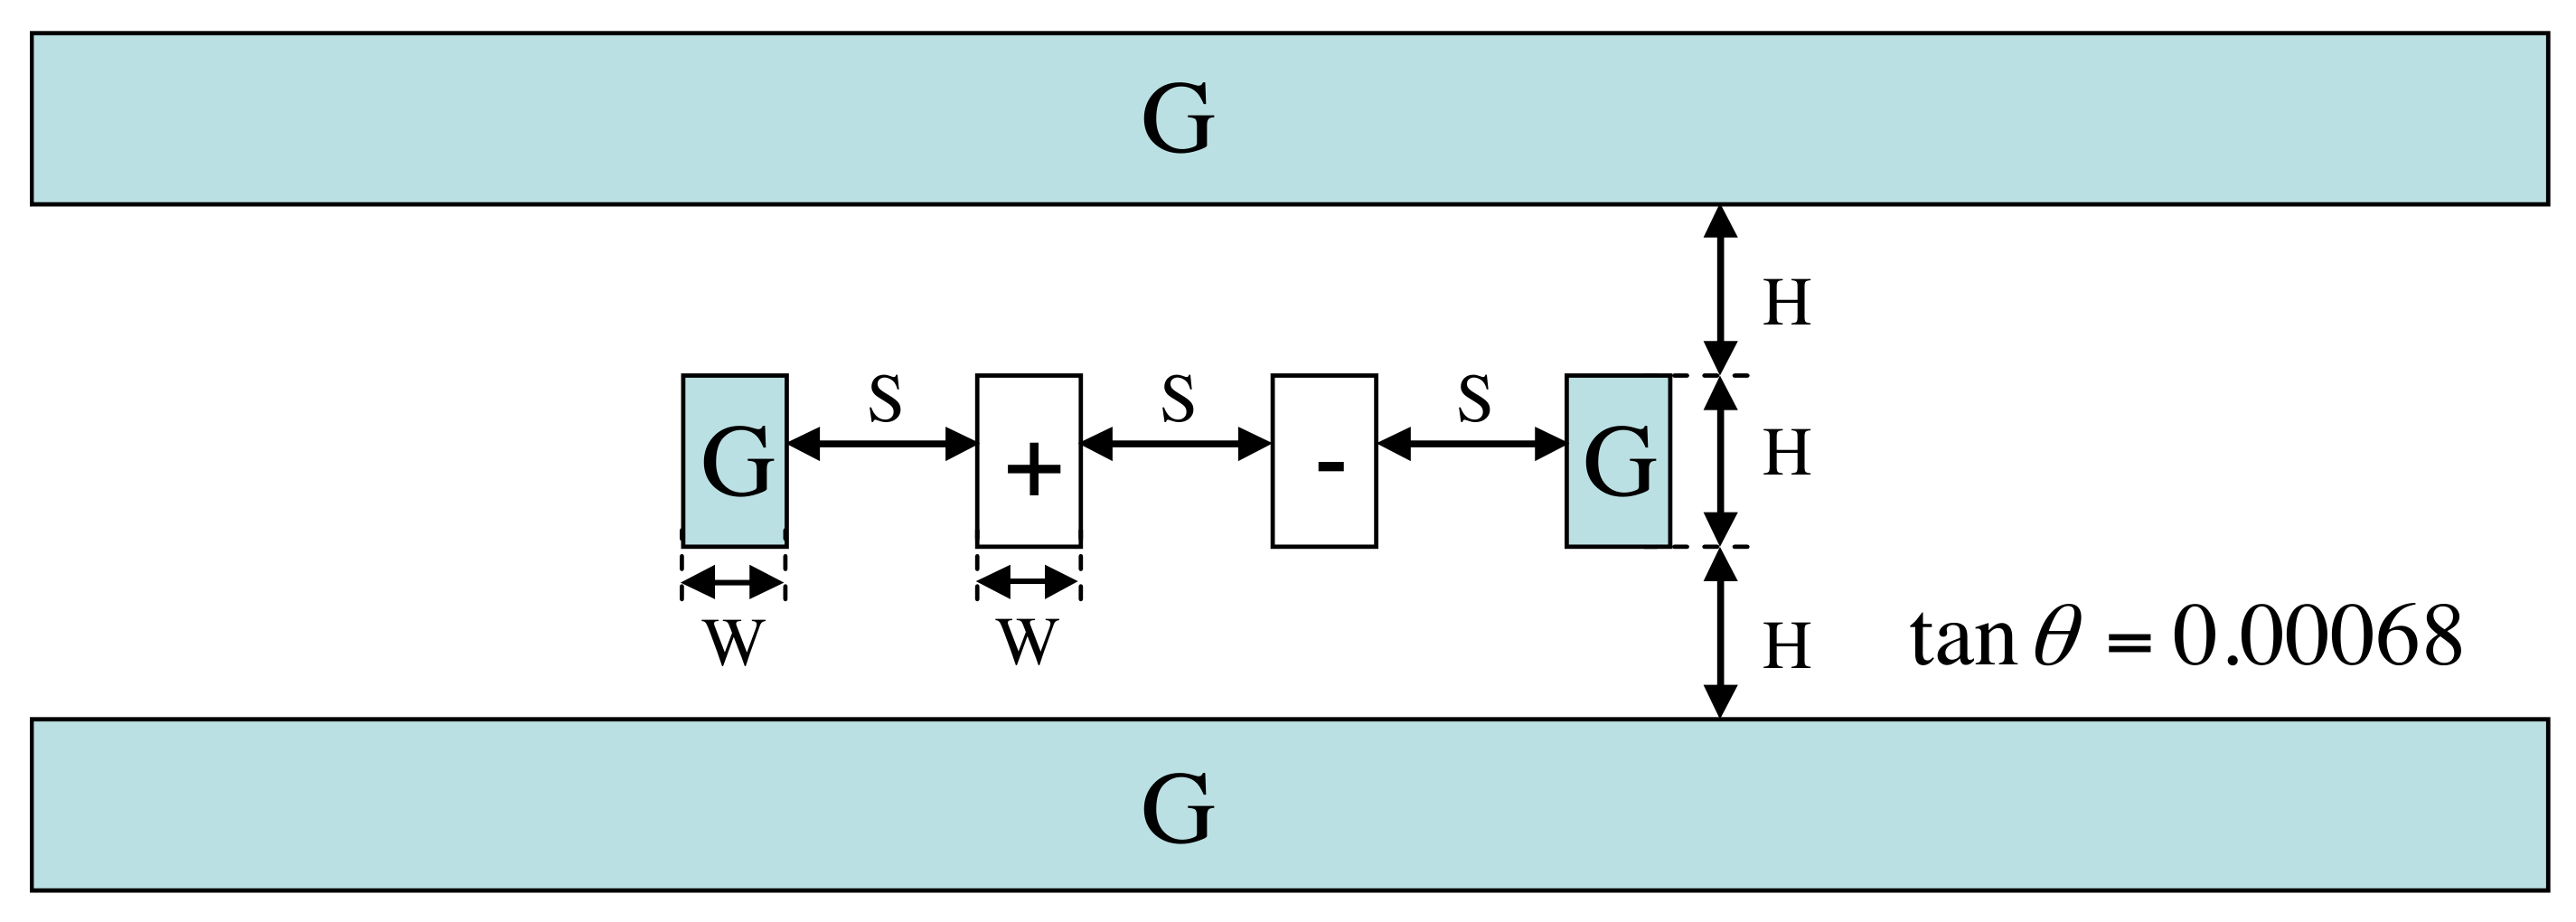
\includegraphics[width=0.95\linewidth]{Figures/Rep3TransmissionLine.png}
	\caption{Cross section of a differential stripline, Source: \cite{zhang2009high}.} 
    \label{fig:rep3:crosssection}
\end{figure}
% Transmission line geometries:
% The length of the global communication in this paper is set to \textit{5 mm}.
According the ITRS roadmap the wire thickness and width ratio should be 2 (see: \cref{fig:rep3:crosssection}).
Larger spacings (S) let the characteristic impedance ($Z_{0}$) increase, which reduces the attenuation and hence gives better eye-diagram performance. %3) Delay and power models ==>> NOT WRITTEN ANYTHING, DO NOT SEE THE USE
% The spacing is varied so that $S = 0.5H, H, 1.5H and 2H$

% B. Transceiver design and modeling
The transceiver stage sense amplifier is based on the same sense amplifier as in \cref{ss:schinkel2009low}.
This design is chosen due to its flexibility to balance the performance metrics.
Simulations have shown that the termination resistance ($R_{l}$) and ($R_{d}$) are dominant in the power consumption.

%Problem formulation and optimization flow
To find the optimum passive compensation for high speed compensation four parameters are optimized: $R_{l}$, $R_{d}$, $C_{d}$ and $R_{s}$.
Here $R_{s}$ is the output resistance of the inverter chain output.
It has to be optimized to minimize the sense amplifier delay.

This optimization problem is constrained as a non-linear programming problem and uses \acc{sqp} to solve it.
The global design goals are to minimize: latency (\textbf{min-d}), latency-power product (\textbf{min-dp}) and the $latency^{2}$-power product (\textbf{min-ddp}).
% global explanation of optimizaiton work flow
The optimization flow inputs are the technology node and wire dimensions.
Then the wire and transceiver model are build respectively.
In each iteration the delay and power parameters of the wire are derived after which the step response of the T-line is simulated.
Based on this the eye opening is determined.
Given the design goals the cost function is evaluated by combination of delay and power of both wires and transceivers.
This is utilized by the \ac{sqp} algorithm for optimization.
Finally, the design flow outputs the optimal values.

% Experimental results
The scheme is optimized under the aforementioned design goals and with four different spacings and then compared with repated RC wires (which are also optimized for the different design goals).

For comparison purposes the normalised delay, power and throughput are used which are respectively defined as: $delay_{n} = \frac{\text{propagation delay}}{\text{wire length}}$, $power_{n} = \frac{\text{energy per bit}}{\text{wire length}}$ and $throughput_{n} = \frac{\text{frequency}}{\text{wire pitch}}$.

\begin{figure}	\centering
	
	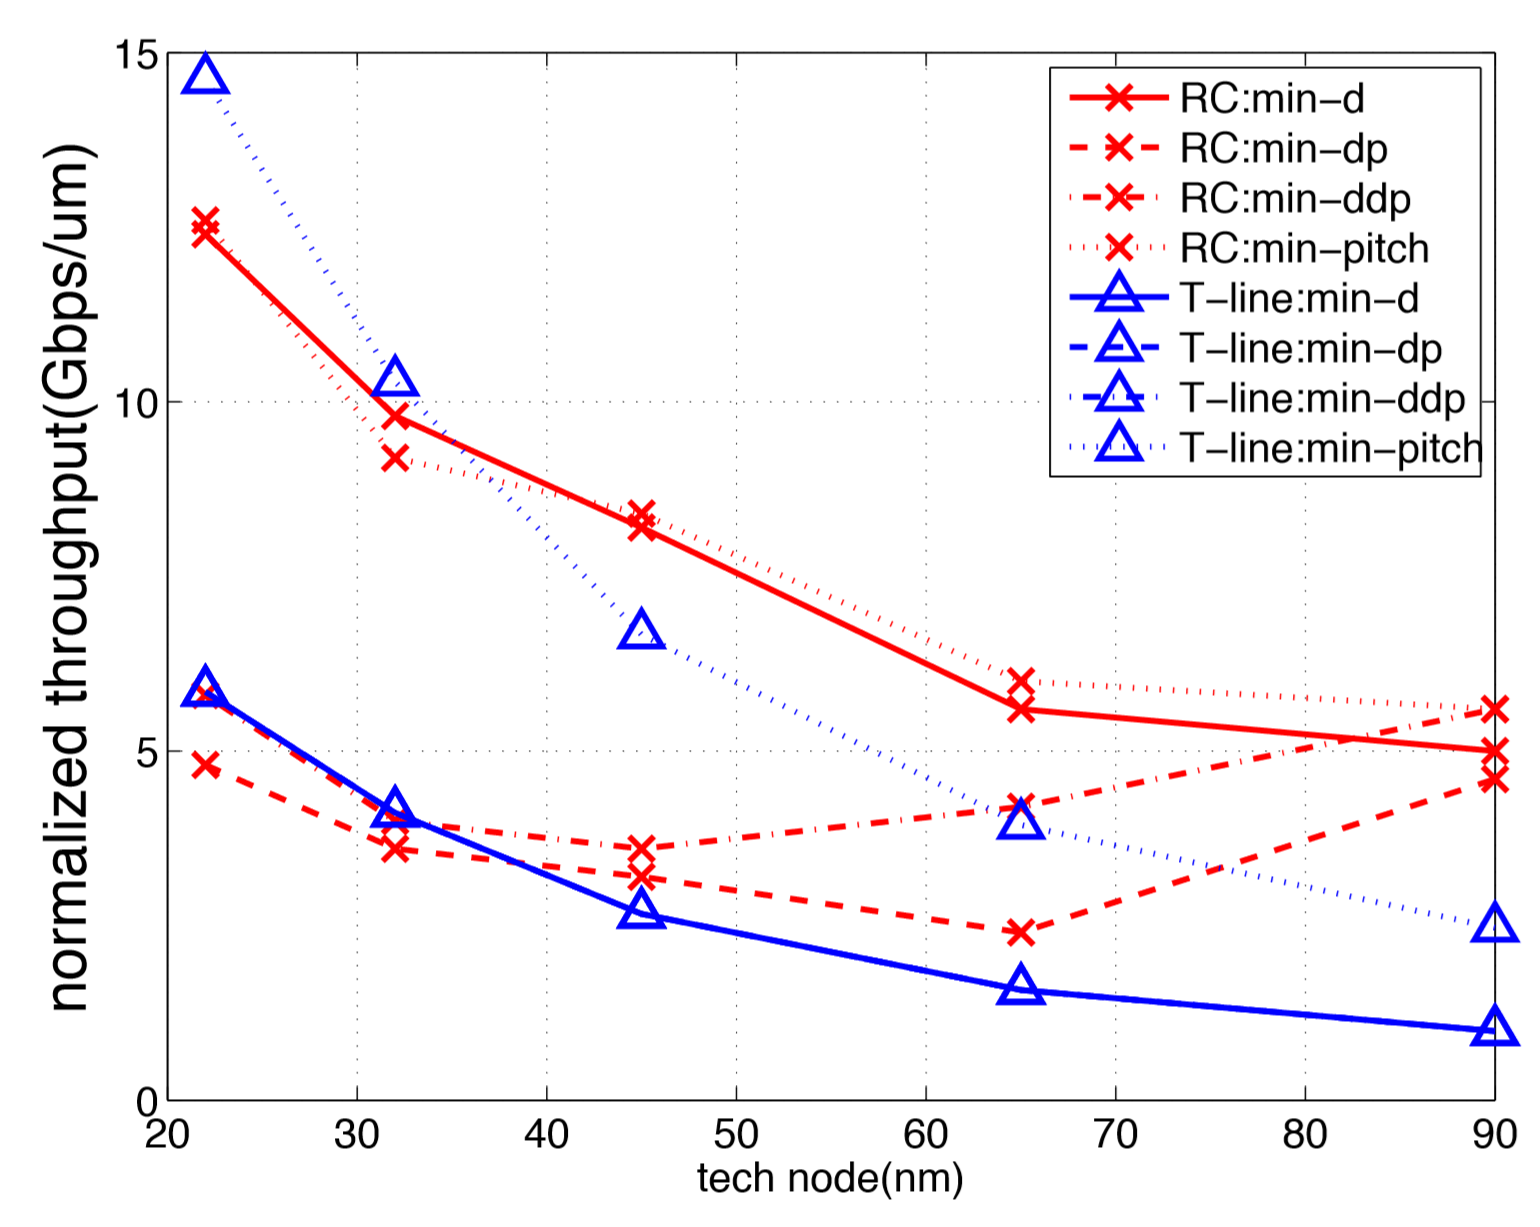
\includegraphics[width=0.95\linewidth]{Figures/Rep3NormThrough.png}
	\caption{Normalized throughput between repeated RC wire and on-chip T-line, Source: \cite{zhang2009high}.} 
    \label{fig:rep3:normthrough}
\end{figure}

The $delay_{n}$ and $power_{n}$ of  \ac{otl} are much better than the RC wire. For $delay_{n}$ from the 60 nm technology node the \ac{otl} performs better.
For $power_{n}$ the \ac{otl} performs better in the whole technology node spectrum.
In \cref{fig:rep3:normthrough} the $throughput_{n}$ is shown with regards to the different optimization criteria.
At \textit{90 nm} technology the RC wire has higher throughput than the \ac{otl}.
The throughput of RC wires decreases due to the usage of smaller repeaters and smaller wire width to reduce the power in the range from \textit{90 nm} to \textit{45 nm}.
In general after the \textit{45 nm} technology the throughput of the schemes is very close, but the throughput of the \ac{otl} is higher.

%conclusion
The wire with the largest spacing (S=2H) gives the optimal results, this is due to higher $Z_{0}$ with reduces the attenuation along the wire.
